\documentclass[border=10pt]{standalone}

\usepackage{tikz}
\usepackage{tikzsymbols}
\usetikzlibrary{calc,patterns,shapes.geometric}

\def\centerarc[#1](#2)(#3:#4:#5){\draw[#1] ($(#2)+({#5*cos(#3)},{#5*sin(#3)})$) arc (#3:#4:#5);}

\begin{document}
	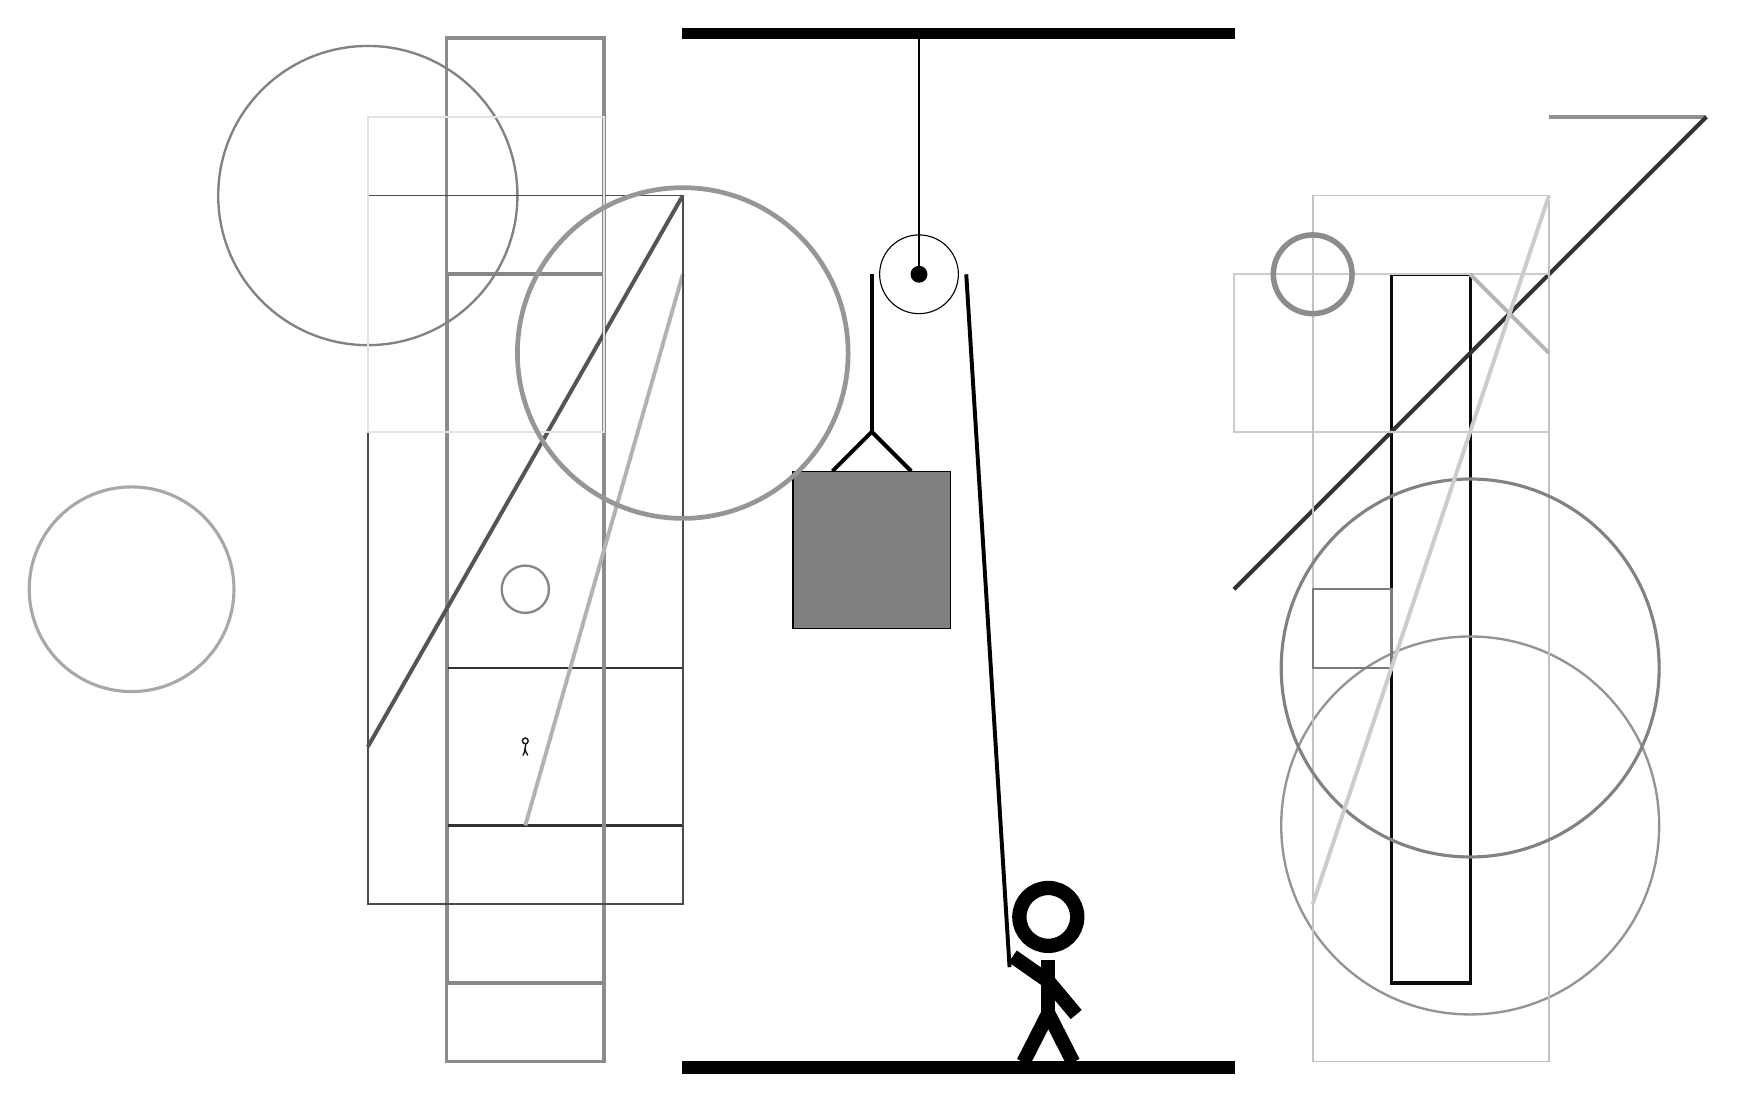
\begin{tikzpicture}
		%%%%% START %%%%%
		
		\draw[fill=black] (-2, 10) rectangle (5, 10.125);
		
		\draw (1, 7) circle (0.5);
		\draw[fill=black] (1, 7) circle (0.1);
		\draw (1, 10) -- (1, 7);
		
		\draw[line width=0.5mm] (-0.1, 4.5) -- (0.4, 5.0) -- (0.9, 4.5);
		\draw[fill=black!50] (-0.6, 4.5) rectangle (1.4, 2.5);
		
		\draw[line width=0.5mm, color=black!47] (-3, 7) rectangle (-5, -2);
		
		\draw[line width=0.3mm, color=black!80] (-2, 0) rectangle (-5, 2);
		\draw[line width=0.5mm, color=black!43](9, 9) -- (11, 9);
		\node[line width=0.4mm, color=black!91] at (-4, 1) {\Strichmaxerl[1][78][81]};
		
		\draw[line width=0.4mm, color=black!96] (7, -2) rectangle (8, 7);
		\draw [line width=0.3mm, color=black!47](-4, 3) circle (0.3);
		\draw[line width=0.5mm, color=black!80](5, 3) -- (11, 9);
		
		\draw [line width=0.4mm, color=black!34](-9, 3) circle (1.3);
		\draw[line width=0.4mm, color=black!45] (-3, -3) rectangle (-5, 10);
		\draw[line width=0.5mm, color=black!30](-4, 0) -- (-2, 7);
		\draw [line width=0.3mm, color=black!42](8, 0) circle (2.4);
		\draw [line width=0.3mm, color=black!49](-6, 8) circle (1.9);
		\draw[line width=0.2mm, color=black!70] (-2, -1) rectangle (-6, 8);
		
		\draw[line width=0.2mm, color=black!20] (5, 7) rectangle (9, 5);
		\draw[line width=0.2mm, color=black!24] (6, 8) rectangle (9, -3);
		\draw[line width=0.5mm, color=black!67](-2, 8) -- (-6, 1);
		\draw[line width=0.5mm, color=black!29](9, 6) -- (8, 7);
		\draw[line width=0.2mm, color=black!11] (-3, 5) rectangle (-6, 9);
		\draw [line width=0.6mm, color=black!41](-2, 6) circle (2.1);
		
		\draw [line width=0.7mm, color=black!45](6, 7) circle (0.5);
		\draw [line width=0.4mm, color=black!49](8, 2) circle (2.4);
		
		\draw[line width=0.3mm, color=black!52] (7, 2) rectangle (6, 3);
		\draw[line width=0.5mm, color=black!20](6, -1) -- (9, 8);
		
		\draw[line width=0.5mm] (0.4, 7) -- (0.4, 5.0);
		\centerarc[line width=0.5mm](1, 7)(0:180:0.6);
		\draw[line width=0.5mm](1.6, 7) -- (2.15, -1.8);
		
		\node at (2.6, -1.9) {\Strichmaxerl[10][-35][-50]};
		
		\draw[fill=black] (-2, -3) rectangle (5, -3.15);
		
		%%%%% END %%%%%
	\end{tikzpicture}
\end{document}